\documentclass
[handout]
{beamer}
\documentclass{beamer}

%%
%%
%%
% From http://tex.stackexchange.com/questions/2072/beamer-navigation-circles-without-subsections
% Solution #2 or 3:
% \usepackage{etoolbox}
% \makeatletter
% % replace the subsection number test with a test that always returns true
% \patchcmd{\slideentry}{\ifnum#2>0}{\ifnum2>0}{}{\@error{unable to patch}}%
% \makeatother
% Solution #1:
\usepackage{remreset}% tiny package containing just the \@removefromreset command
\makeatletter
\@removefromreset{subsection}{section}
\makeatother
\setcounter{subsection}{1}


\usepackage{etex}
\usepackage{pgf}
\usepackage{tikz}
\usepackage{url}
\usepackage{amsmath}
\usepackage{color}
% \definecolor{red}{rgb}{1,0,0}
\usepackage{ulem}
% \usepackage{booktabs}
\usepackage{colortbl,booktabs}
\renewcommand*{\thefootnote}{\fnsymbol{footnote}}
\usepackage{fancybox}
\usepackage[framemethod=TikZ]{mdframed}
\mdfdefinestyle{FactStyle}{%
  outerlinewidth=0.5,
  roundcorner=1pt,
  leftmargin=1cm,
  linecolor=blue,
  outerlinecolor=blue!70!black,
  backgroundcolor=yellow!40
}
\usepackage{cancel}

  \newcommand\Warning{%
    \makebox[2.4em][c]{%
      \makebox[0pt][c]{\raisebox{.2em}{\Large!}}%
      \makebox[0pt][c]{\color{red}\Huge$\bigtriangleup$}}}%

\usepackage{stackengine}
\usepackage{scalerel}
\usepackage{xcolor}
  \newcommand\dangersign[1][2ex]{%
    \renewcommand\stacktype{L}%
    \scaleto{\stackon[1.3pt]{\color{red}$\triangle$}{\tiny !}}{#1}%
  }



\usepackage{dcolumn}
\newcolumntype{d}[1]{D{.}{.}{#1}}

% From
% http://tex.stackexchange.com/questions/109900/how-can-i-box-multiple-aligned-equations
\usepackage{empheq}
\usepackage{tcolorbox}  \newtcbox{\othermathbox}[1][]{%
  nobeforeafter, tcbox raise base, 
  colback=black!10, colframe=red!30, 
  left=1em, top=0.5em, right=1em, bottom=0.5em}

\newcommand\blue{\color{blue}}
\newcommand\red{\color{red}}
\newcommand\green{\color{green!75!black}}
\newcommand\purple{\color{purple}}
\newcommand\bluegreen{\color{blue!75!green}}
\newcommand\orange{\color{orange}}
\newcommand\redgreen{\color{red!50!green}}
\newcommand\grey{\color{black}}
\newcommand\gap{\vspace{.1in}}
\newcommand\nb{${\red\bullet}\ $}
\newcommand\halfgap{\vspace{.05in}}
\newcommand\divideline{\line(1,0){352}}
\usepackage{marvosym} % for \Smiley

\newcommand{\bluealert}[1]{{\blue\textbf{#1}}}

% \usepackage{beamerthemesplit} %Key package for beamer
\usetheme{Singapore}
% \usetheme{Szeged}
% \usetheme{Garfield}
% \usetheme{CambridgeUS}
% \usenavigationsymbolstemplate{} %Gets rid of slide navigation symbols


\setbeamercolor{separation line}{use=structure,bg=structure.fg!50!bg}
% \begin{beamercolorbox}[colsep=0.5pt]
%   {upper separation line foot}
% \end{beamercolorbox}



\makeatletter
\setbeamertemplate{footline}
{
  \leavevmode%
  \hbox{%
% \begin{beamercolorbox}[colsep=0.5pt]
%   {upper separation line foot}
% \end{beamercolorbox}


  \begin{beamercolorbox}[wd=.5\paperwidth,ht=2.25ex,dp=2ex,colsep=0.5pt]%
    {upper separation line foot}
    \usebeamerfont{author in head/foot}%
    \hspace*{2ex}\insertshortdate:\ \insertshorttitle
  \end{beamercolorbox}%
  \begin{beamercolorbox}[wd=.5\paperwidth,ht=2.25ex,dp=2ex,right]{title in head/foot}%
    \usebeamerfont{title in head/foot}
    {\insertshortauthor}\hspace*{2ex}
  \end{beamercolorbox}}%
  % \begin{beamercolorbox}[wd=.333333\paperwidth,ht=2.25ex,dp=2ex,right]{date in head/foot}%
  %   \usebeamerfont{date in head/foot}\insertshortdate{}\hspace*{2em}
  %   \insertframenumber{} / \inserttotalframenumber\hspace*{2ex} 
  % \end{beamercolorbox}%
  \vskip0pt%
}
\makeatother

\usetikzlibrary{decorations.markings}
\usetikzlibrary{arrows}


\title{Final Exam Review}
\author{Peter Garfield, UCSB Mathematics}
\date{March 15, 2017}
%\institute{}


\useinnertheme{default}

\usefonttheme{serif}
% \usecolortheme{rose}
% \usecolortheme{whale}
% \usecolortheme{orchid}
\usecolortheme{crane}
% \usecolortheme{dolphin}


%TEMPLATE
\setbeamertemplate{navigation symbols}{}

\setbeamertemplate{note page}[compress]

\setbeamertemplate{frametitle}{
  \vspace{0.5em}
  % \begin{centering}
  {\huge\blue\textbf{\textmd{\insertframetitle}}}
  \par
  % \end{centering}
}

% From http://tex.stackexchange.com/questions/7032/good-way-to-make-textcircled-numbers:
\newcommand*\circled[1]{\tikz[baseline=(char.base)]{\node[shape=circle,draw,fill=orange,inner sep=1pt] (char) {#1};}} 
% \renewcommand{\labelenumi}{\circled{\textbf{\arabic{enumi}}}}

\let\olddescription\description
\let\oldenddescription\enddescription
\usepackage{enumitem}
\let\description\olddescription
\let\enddescription\oldenddescription

% \usepackage[loadonly]{enumitem}
\setlist[enumerate,1]{label=\colorbox{orange}{\arabic*.},font=\bfseries}
%\setlist[enumerate,2]{label=\colorbox{blue!25}{(\alph*)},font=\bfseries}
% \setlist[enumerate,1]{label=\arabic*.,font=\bfseries}
\setlist[itemize,1]{label=\red$\bullet$}
\setlist[itemize,2]{label=\blue$\bullet$}

\newcommand\answer[1]{\fbox{#1}}
% \renewcommand\answer[1]{}

\newcommand{\antilog}{\operatorname{antilog}}








\title{}
\title{Calculus Intro}
\date{May 5, 2022}


\begin{document}
\small



\section*{Administration}

\frame{
  \frametitle{}
  {\Huge{}Welcome Back!}\\[.5em]

  {\Huge{}Differential Calculus}
  \vfill
  {\Large{}Instructor:}\\
  \ \hspace*{0.2in} Nathan Schley ({\it Sh}+{\it lye}), \url{schley@math.ucsb.edu}\\
  \ \hspace*{0.2in} South Hall 6701
  \\[0.5em]

  {\Large{}Office Hours:}\\
  \ \hspace*{0.2in} T R 11-11:50, T 3:45-4:35 Details on Gauchospace. 
  \bigskip

  \copyright\ 2022\ Daryl Cooper, Peter M.\ Garfield, Ebrahim Ebrahim \& Nathan Schley\\
  Please do not distribute outside of this course.
  \vfill

}


\section*{Review}

\frame{
  \frametitle{Graphical Approach}

  \begin{minipage}{0.5\linewidth}
    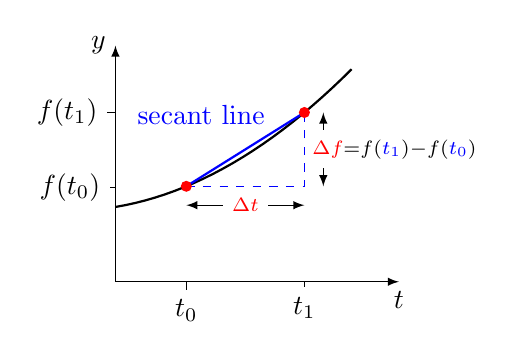
\begin{tikzpicture}[x=12mm,y=12mm,>=latex]
        \draw[black,->] (0,0) -- (3,0) node[below] {$t$};
        \draw[black,->] (0,0) -- (0,2.5) node[left] {$y$};
        % Ticks:
        \draw[thin,black] (0.75,0) -- (0.75,-3pt) node[below] {$t_0$};
        \draw[thin,black] (2,0) -- (2,-2pt) node[below] {$t_1$};
        \draw[thin,black] (0,1) -- (-2pt,1) node[left] {$f(t_0)$};
        \draw[thin,black] (0,{0.75+(2+1/2)^2/6}) -- (-3pt,{0.75+(2+1/2)^2/6}) node[left] {$f(t_1)$};
        \draw[black,thick] plot[domain=0:2.5] (\x,{0.75+(\x+1/2)^2/6});
      %
        \draw[thick,blue] (0.75,{0.75+(0.75+1/2)^2/6}) -- (2,{0.75+(2+1/2)^2/6}) node[near end,left,yshift=2mm] {secant line};
        \draw[thin,black,<->] (0.75,{0.75+(0.75+1/2)^2/6-0.2}) -- (2,{0.75+(0.75+1/2)^2/6-0.2}) node[midway,red,fill=white] {$\scriptstyle\Delta t$};
        \draw[thin,black,<->] (2.2,{0.75+(0.75+1/2)^2/6}) -- (2.2,{0.75+(2+1/2)^2/6}) node[midway,fill=white,right,xshift=-0.75em] {$\scriptstyle{\red\Delta f}=f({\blue t_1})-f({\blue t_0})$};
        \draw[thin,blue,dashed] (0.75,{0.75+(0.75+1/2)^2/6}) -- (2,{0.75+(0.75+1/2)^2/6}) -- (2,{0.75+(2+1/2)^2/6});
        % 
      %
        \fill[red] (0.75,{0.75+(0.75+1/2)^2/6}) circle (2pt);
        \fill[red] (2,{0.75+(2+1/2)^2/6}) circle (2pt);
    \end{tikzpicture}
  \end{minipage}
  \hfill
  \parbox{50mm}{%
    ${\red\Delta f}=$ change in $f$ \\
    ${\red\Delta t}=$ change in $t$\\[0.5em]
    \alert{Many ways to say same thing:}\\
    $\begin{array}{l}
       \left(\begin{array}{c} \text{{\blue average} rate of}\\ \text{change of $f$}\end{array}\right)  = \dfrac{\text{change in $f$}}{\text{change in $t$}}\\
       = \dfrac{\red \Delta f}{\red\Delta t}\\
       =  \text{slope of {\blue secant line}}
       = \dfrac{f({\blue t_1})-f({\blue t_0})}{{\blue t_1}-{\blue t_0}}
     \end{array}$
   }
   \pause

   The derivative is defined to be
   \begin{equation*}
     \lim_{\Delta t\to0} \left(\frac{\red\Delta f}{\red\Delta t}\right) 
     = \frac{df}{dt}
   \end{equation*}
   \pause

   Idea: As $t_1$ moves closer to $t_0$ the secant line approaches the {\blue tangent line}  at $t_0$.
   This is the line with the {\blue same slope} as the graph at $t_0$.

   % \fbox{{\red Let's watch a movie }} \qquad\qquad  No, not  {\blue The Bourne Identity}  :(\\

   % http://www.youtube.com/watch?v=AdQG2iSLDjA\\
   % http://www.youtube.com/watch?v=s3q8D79bjiE\&feature=related
}


\frame{
  \frametitle{Understanding Derivatives}

  There are many ways to {\blue think} about derivatives.  You {\blue
    need} to understand these to apply to problems. 
  \gap
  \gap 

  \begin{minipage}{0.35\linewidth}
    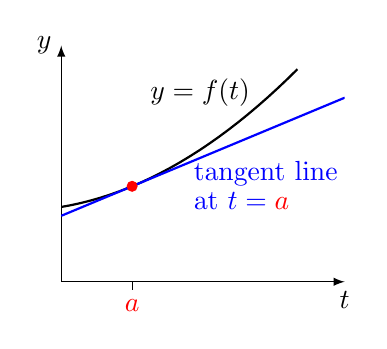
\begin{tikzpicture}[x=12mm,y=12mm,>=latex]
        \draw[black,->] (0,0) -- (3,0) node[below] {$t$};
        \draw[black,->] (0,0) -- (0,2.5) node[left] {$y$};
        % Ticks:
        \draw[thin,black] (0.75,0) -- (0.75,-3pt) node[below] {\red$a$};
        % \draw[thin,black] (2,0) -- (2,-2pt) node[below] {$t_1$};
        % \draw[thin,black] (0,1) -- (-2pt,1) node[left] {$f(t_0)$};
        % \draw[thin,black] (0,{0.75+(2+1/2)^2/6}) -- (-3pt,{0.75+(2+1/2)^2/6}) node[left] {$f(t_1)$};
        \draw[black,thick] plot[domain=0:2.5] (\x,{0.75+(\x+1/2)^2/6});
        \begin{scope}
          \clip (0,0) rectangle (3,2.5);
          \draw[blue,thick] plot[domain=0:3] (\x,{(0.75+1/2)*(\x-0.75)/3+0.75+(0.75+1/2)^2/6});
          \node[blue,right] at (1.3,1.15) {tangent line};
          \node[blue,right] at (1.3,0.85) {at $t={\red{}a}$};
          \node[left] at (2.1,2) {$y=f(t)$};
        \end{scope}
      %
      %
        \fill[red] (0.75,{0.75+(0.75+1/2)^2/6}) circle (2pt);
    \end{tikzpicture}
  \end{minipage}
  \hfill
  \parbox{60mm}{%
    slope of {\blue graph} at {\red a}\\
    = slope of {\blue tangent line} \\%\small{\red $\quad\quad^{discuss}$}\\
    = {\purple instantaneous rate of change} of $f$ at ${\red a}$\\
    \\
    $= \left(
      \begin{array}{l}
        \text{limit of average rate of change } \\ 
        \text{of $f$ over shorter and shorter}\\
        \text{ time intervals starting at\ {\red$a$}}
      \end{array}
    \right)$\\
    \\
    $=$ limit of slopes of secant lines\\
    $= f'({\red a})\ =\ \left. \dfrac{df}{dt}\right|_{t={\red a}}$
  }

}




\section*{Interpreting Derivatives}

\frame{
  \frametitle{The Importance of Units}


  \begin{minipage}{0.4\linewidth}
    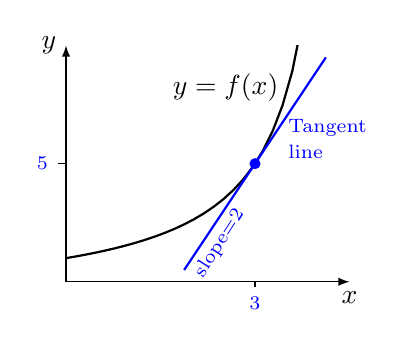
\begin{tikzpicture}[x=12mm,y=6mm,>=latex]
      \draw[black,->] (0,0) -- (3,0) node[below] {$x$};
      \draw[black,->] (0,0) -- (0,5) node[left] {$y$};
      % Ticks:
      \draw[thin,black] (2,0) -- (2,-2pt) node[below,blue] {$\scriptstyle3$};
      \draw[thin,black] (0,2.5) -- (-3pt,2.5) node[left,blue] {$\scriptstyle5$};
      \begin{scope}
        \clip (0,0) rectangle (3,5);
        \draw[black,thick] plot[domain=0:2.5] (\x,{-0.5-3/(\x-3)});
      \end{scope}
      \node[left] at (2.35,{-0.5-3/(2.35-3)}) {$y=f(x)$}; 
      \fill[blue] (2,{-0.5-3/(2-3)}) circle (2pt);
      % Tangent line to y=-0.5-3/(x-3), so y'=3/(x-3)^2 = 3 at x=2.
      % so through (2,2.5) with slope 3; y=3x-3.5
      \draw[thick,blue] (1.25,0.25) -- (2.75,4.75);
      \node[rotate=57.5,blue] at ({1.5+1*0.125},{1-1.5*0.125}) {$\scriptstyle\text{slope}=2$};
      \node[right,blue] at (2.25,3.25) {$\scriptstyle\text{Tangent}$};
      \node[right,blue] at (2.25,2.75) {$\scriptstyle\text{line}$};
    \end{tikzpicture}
  \end{minipage}
  \hfill
  \begin{minipage}{60mm}
    Told $f({\blue 3}) = 5$ and $f{\green '}({\blue 3})={\green 2}$
    \gap

    This means the slope of the tangent line to the graph $y=f(x)$ at $x=3$ is $2$.
    \gap 

    The derivative is this slope, so\ldots
    \gap 

    \fbox{The {\blue units}\ of $\dfrac{dy}{dx}$\ are $\dfrac{\text{units of y}}{\text{units of x}}$}
  \end{minipage}
  \bigskip
  \pause

  \alert{Examples:}

  Heating: derivative units are $\$/{}^{\circ}\ \text{F} = \text{dollars per degree F}$

  Adrenaline: $\text{bpm}/\text{mg} = \text{beats per minute per mg of adrenaline}$.
  \gap

  Units help you understand the {\blue meaning} of the derivative.

}



\frame{
  \frametitle{Interpretation of Derivatives I}

  Suppose $f({\red x})=$ the {\blue percentage of children who still
    get measles} when ${\red x}\%$ of children are inoculated. 
  \gap 

  \alert{Question:}\ Which of the following is a plausible value for $f'(40)$?
  \begin{center}
    A$=0$
    \quad 
    B$= 2$
    \quad 
    C$ = 50$
    \quad 
    D$= -2$
    \quad 
    E$ = -50$
    \pause
    \quad 
    \fbox{D} 
  \end{center}
  \pause
  \gap 

  \alert{Question:}\ If $f({\red 40})={\blue 20}$ and $f'({\red
    40})=-2$, which must be true?
  \begin{itemize}
  \item[A] when 20\% of children are inoculated the  percentage who
    gets measles decreases by $2$\%

  \item[B] when 20\% of children are inoculated then inoculating an
    extra 1\% of children would reduce the number of measles cases by
    another 2\%

  \item[C] If the inoculation rate is 41\% then 18\% of children gets
    measles

  \item[D] If the inoculation rate is 20\% then 2\% fewer cases of
    measles arise if an extra 1\% of children can be inoculated

  \item[E] none of the above
  \pause
  \hfill\alert{Answer:}\ \fbox{C}

  \end{itemize}
}


\frame{
  \frametitle{Interpretation of Derivatives II}

  Air temperature gets colder the higher you go.\\
  $T({\red x})=$ {\blue air temperature} in $^{\circ}C$ at a height $\red x$ meters above sea level.

  \alert{Question:}\ Which of these is a plausible value for $T'({\red 2000})$?
  \begin{center}
    A$ = -1$
    \quad 
    B$ = 1$
    \quad 
    C$ = 0$
    \quad 
    D$ = 1/200$
    \quad 
    E$ = -1/200$
    \pause
    \quad
    \fbox{E} 
  \end{center}
  \pause
  \gap 

  \alert{Question:}\ If $T({\red 2000})={\purple 10}$ and $T{\red'}({\red 2000})=-{\bluegreen 1/200}$, which is most plausible?
  \begin{itemize}
  \item[A] the temperature at sea level is $16^oC$
  \item[B] the temperature $2400$ meters above sea level is $8^oC$
  \item[C] the temperature $10$ meters above sea level is $2000^oC$
  \item[D] 2000 meters above sea level the temperature is decreasing at a rate of $1/200^oC$ per minute.
  \item[E] none of these are plausible
  \end{itemize}
  \pause
  \alert{Answer:}\ \fbox{B}


}



\frame{
  \frametitle{Interpretation of Derivatives III}
  \vspace*{-0.30in}

  \begin{align*}
    {\red x} 
    & = \text{money spent (in thousands of \$) in one month on advertising.}\\
    {\blue f(x)}
    & = \text{{\blue sales} (in thousands of \$) in a month when ${\red x}$ is spent on advertising.}
  \end{align*}
  \pause\vspace*{-0.2in}

  \alert{Question:}\ If $f({\red 20})={\blue 60}$ and $f{\red'}({\red 20})=3$ which must be true?
  \begin{itemize}
  \item[A] When the sales of the company are 20 thousand dollars in
    one month the amount spent on advertising is increasing at a rate
    of 3 thousand dollars per month

  \item[B] When the company spends 20 thousand dollars per month on
    advertising the sales rise at a rate of 3 thousand dollars per
    month 
  \item[C] When the company spends 20 thousand dollars per month on
    advertising each extra dollar a month spent on advertising
    generates an extra 3 dollars of sales. 

  \item[D] When the company spends 3 thousand dollars per month on
    advertising the sales are increasing at a rate of 20 thousand
    dollars per month 

  \item[E] None of the above
    \pause
    \hfill
    \alert{Answer:}\ \fbox{C}
  \end{itemize}

}


\section*{Exam Info}

\frame{
  \frametitle{Midterm 2: Next Tuesday}

  {\Large\color{blue}Bring:}
  \begin{itemize}
  \item A pen or \alert{sharp} pencil.
  \item A $3"\times5"$ card with your notes. 
  \item Student ID. (Verify your midterm1 ID if haven't)
  \end{itemize}
  \bigskip

  {\Large\color{red}Don't bring:}
  \begin{itemize}
  \item A calculator
  \end{itemize}
  \smallskip

  Please Be Early! 

  There are sample exam questions on Gauchospace.\\
  Some of them are from an old Midterm 2, and the rest are a few extra to round out your practice. 
  
  The exam is cumulative.

}


\section*{Some Practice Exam Problems}

\frame{\huge
Write out the following sum:
$$ \sum_{i=2}^7 (i^2 + 3). $$
}

\frame{
These review problems put together different ideas you have been reviewing. 
\begin{itemize} 
\item For the function $f(t)$, find the average rate of change between $t=3$ and $t=5$. \pause 
\item Find the average rate of change between $t=3$ and $t=3+h$. \pause 
\item Simplify your answer to the last problem. \pause
\item What is the limit as $h$ approaches 0? \pause 
\item what is the instantaneous speed of $f$ at 3? 
\end{itemize}
}

\frame{\huge
Given that $\log(2)$ is approximately $0.3$, try to estimate $\log(5)$.\\
(Hint: $5=10/2$).
}

\frame{\large
There are 4 grams of gold.\\[1em]
How many grams of silver should be mixed with this gold to create a mixture that is x\% gold?
}


\frame{
A garden is in the shape of a square and with a semicircle on one side.  The length of each side of the square is $t$, and the area of the garden is $A$.
Express $t$ in terms of $A$, then express the perimeter of the garden in terms of $A$.
\begin{center}
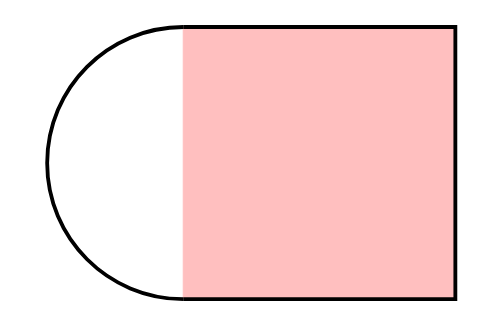
\includegraphics[scale=0.3]{garden.png}
\end{center}
}


\frame{\large
A growing rectangle doubles its length and width every three hours. By what factor has its area changed after one day?
}


\frame{\large
A population of bacteria is growing exponentially.
At one time it is found to be 10 mg in mass, and exactly one day later it is found to be 100 mg in mass.
What is the doubling time in hours? That is, how long does it take for the bacteria population to double? (Hint: $\log(2) \approx .3$)
\\[1em]
How long after there are 100 mg will there be 1 gram of bacteria?
}

\frame{\large
A population of mice is getting killed off by a disease.
The disease is dormant in all mice of the population, and it seems to kill them off at random, giving each mouse an equal chance of dying each day.
Sadly, the mouse population decays exponentially.
At one time there were a million mice, and 20 days later there are only 100 remaining.
What is the half-life of the mouse population? That is, how long does it take for half of the mice to die?
\\[1em]
How long after the 20 days will there be only one mouse left?
}



% \frame{
% The following table shows the temperature throughout a particular day:
% \begin{center}
% \begin{tabular}{|l|r|r|r|r|r|r|r|}
% \hline
% time           & 7:00 & 8:00 & 9:00 & 10:00 & 11:00 & 12:00 & 1:00 \\ \hline
% $^\circ\text{C}$ & 5    & 4    & 8    & 8     & 12    & 14    & 15   \\ \hline
% \end{tabular}
% \end{center}
% From 9:00 to 12:00, what is the average rate of change of the temperature? Include units in your answer.
% }



\frame{\huge
Solve for $x$:
$$ \log(-x+5)=23 $$
}





\end{document}


